%!TEX root = ./report.tex

\section{Dynamic Programming}
The weights for the tracking and the obstacle avoidance cost are set to the values provided in the code comments.
In particular, the weights are set to
\begin{eqnarray}
	\omega_{track-d} &=& 10\, ,\\
	\omega_{track-heading} &=& 20\, ,\\
	\omega_{collision-avoidance} &=& 100 \, .
\end{eqnarray}
\subsection{Experiments}
Figure~\ref{fig:dyn_prog_results} shows the results for two different paths with obstacle avoidance disable (left) and enabled, respectively.
Obviously, the obstacle avoidance does indeed produces collision free paths with the weights given above.
As the cost decays cubically with the distance to an obstacle the vehicle still might pass close by obstacle, but does not collide.
For instance, consider the obstacle at $(17, 54)$ in Figure~\ref{fig:dyn_prog_results}~(d).
The visualization is a bit misleading, but in fact the vehicle does not collide, but passes by the obstacle in a distance of approximately $0.5m$.

\begin{figure}[h]
	\begin{subfigure}{.49\textwidth}
		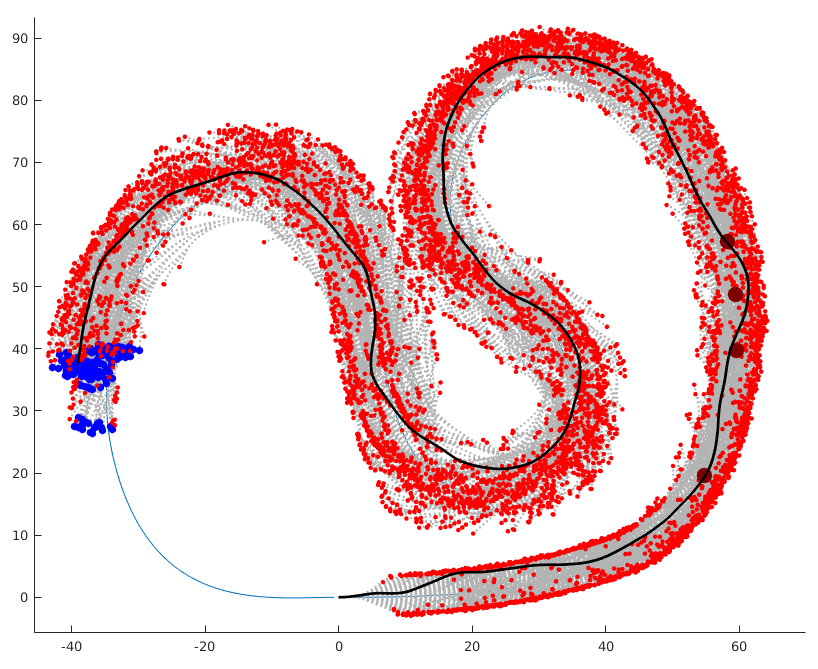
\includegraphics[width=\textwidth]{figures/dyn_prog_no_obs_avoid.png}
		\subcaption{No obstacle avoidance, path 3}
	\end{subfigure}
	\begin{subfigure}{.49\textwidth}
		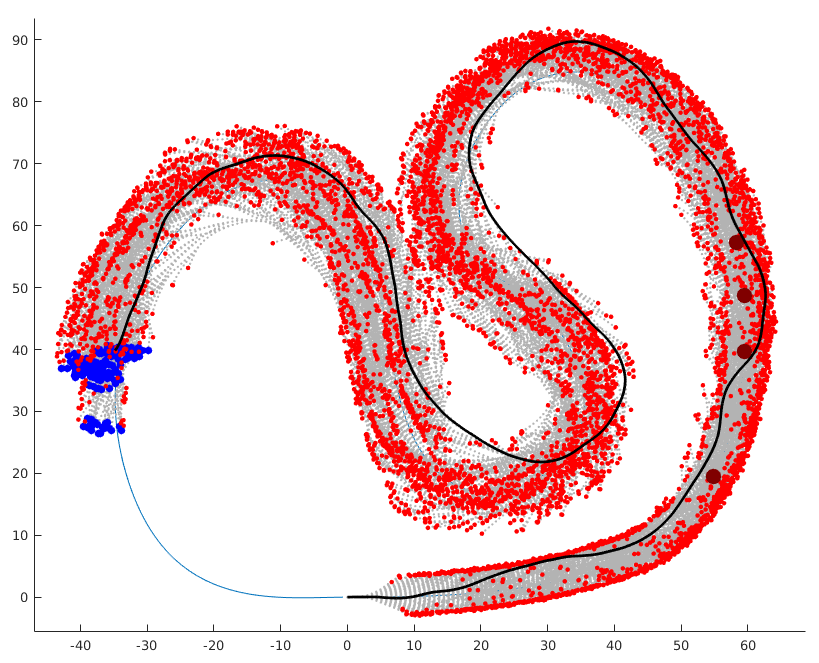
\includegraphics[width=\textwidth]{figures/dyn_prog_obs_avoid.png}
		\subcaption{Obstacle avoidance, path 3}
	\end{subfigure}
	\begin{subfigure}{.49\textwidth}
		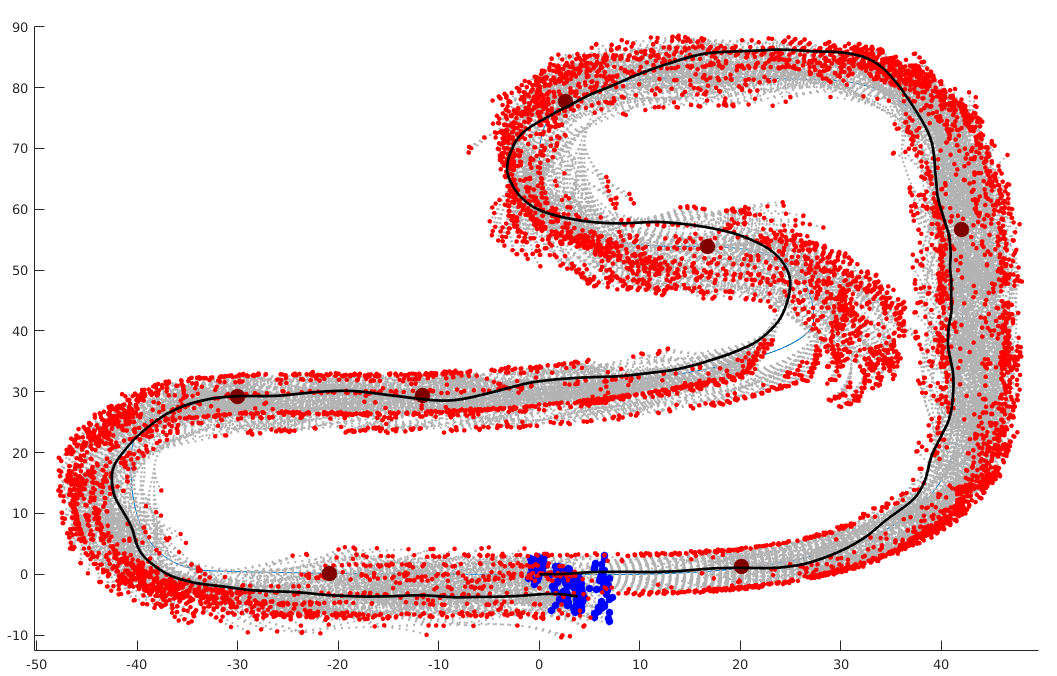
\includegraphics[width=\textwidth]{figures/dyn_prog_no_obs_avoid_2.png}
		\subcaption{No obstacle avoidance, path 2}
	\end{subfigure}
	\begin{subfigure}{.49\textwidth}
		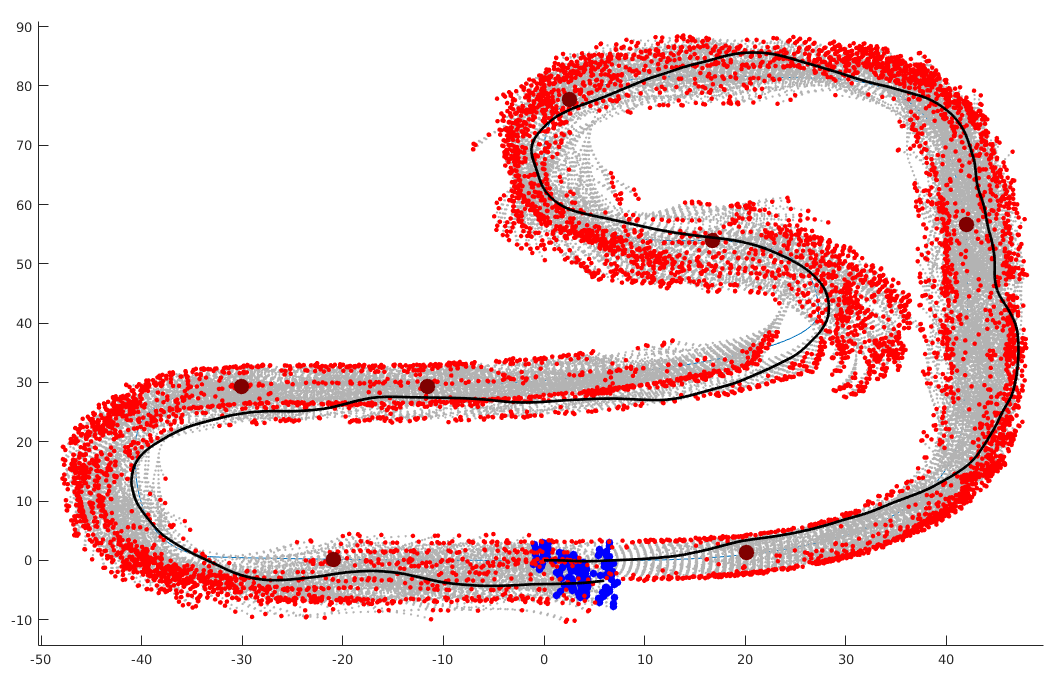
\includegraphics[width=\textwidth]{figures/dyn_prog_obs_avoid_2.png}
		\subcaption{Obstacle avoidance, path 2}
	\end{subfigure}
	\caption{Performance of the dynamic programming approach for path tracking. On the left the obstacle avoid is disables ($\omega_{obs} = 0$) and on the right it is activated with cost $\omega_{obs} = 100$.}
	\label{fig:dyn_prog_results}
\end{figure}

\subsection{Does it Always Find a Collision-free Path?}
\paragraph{Short answer:} No.

\paragraph{Long answer:} First, one needs to define the term \emph{collision free}.
In the setting here, all obstacles are points and are infinitely small.
Therefore, a path is collision free if it will not pass \emph{exactly} through an obstacle in the setting here.
It seems quite hard to pass \emph{exactly} through an obstacle and so it should be easy to find non-colliding trajectories.
However, as shown below it quite easy to construct settings, where no collision-free path can be found.

Note that for a finite amount of nodes in the graph there is only a finite amount of possible control actions, as the control actions to get to the next state are picked from the fixed and finite set of possible control actions $\Omega$.
Therefore, one can easily construct settings where the algorithm can not find a collision-free solution by picking a time $t$ and placing an obstacle at all the places the vehicle can be at that time given the fixed set of control actions $\Omega$.
One such construction is to pick $t=0$ and placing an obstacle at the starting position of the vehicle.
Then, every node cost will be infinite and the dynamic programming approach can never find a collision-free path in this case.

\subsection{Why Randomization?}

\subsection{Discussion}

